% Nama Kelompok : 
% Kelas : D4 TI 1A
% Anggota : 
% 1. Harun    1174027
% 2. Fahmi    1174021
% 3. Kukuh    1174016
% 4. Izza    1174013
% 5. Rizal    1174014
% 6. Lawimner 1174030



\documentclass{article}
\usepackage{graphicx}
\begin{document}
Artikel ini berisi tentang Tugas Arduino
	
  \begin{figure}[ht]
  \centerline{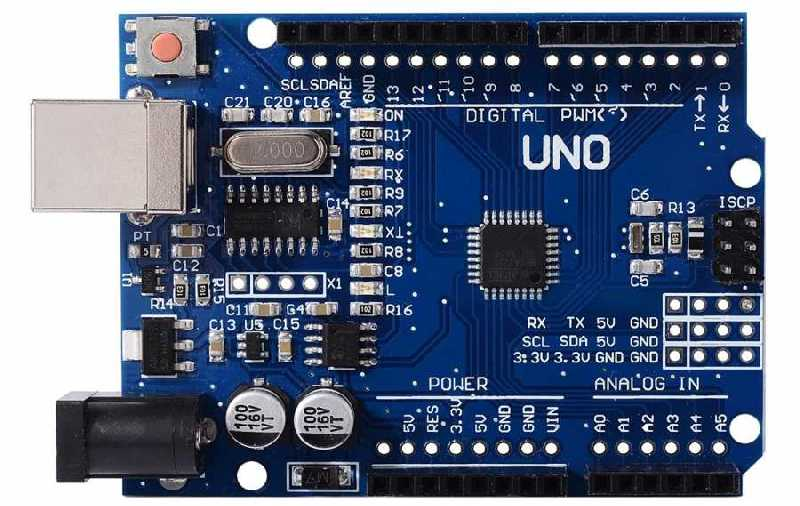
\includegraphics[width=1\textwidth]{../figures/arduino10.jpg}}
  \caption{Ini adalah Arduino}
  \label{arduino}
  \end{figure}

\section{Pengertian Arduino Uno}
\ref{arduino}Arduino adalah pengendali mikro single-board yang bersifat open-source, diturunkan dari Wiring platform, dirancang untuk memudahkan penggunaan elektronik dalam berbagai bidang. Arduino UNO merupakan sebuah board mikrokontroler yang dikontrol penuh oleh ATmega328.

\section{Kegunaan Arduino Uno}
Arduino dapat disambungkan dan mengontrol led, beberapa led, bahkan banyak led, motor DC, relay, servo, modul dan sensor-sensor, serta banyak lagi komponen lainnya.
Karena itu kami kelompok 3 ingin membuat sensor untuk lampu led . Berikut proses dan alat pembuatannya:

\section{Alat}
Untuk membuat Alat sensor LED yang kita butuhkan adalah :
 1. Arduino Uno
 \ref{arduino}
  \begin{figure}[ht]
  \centerline{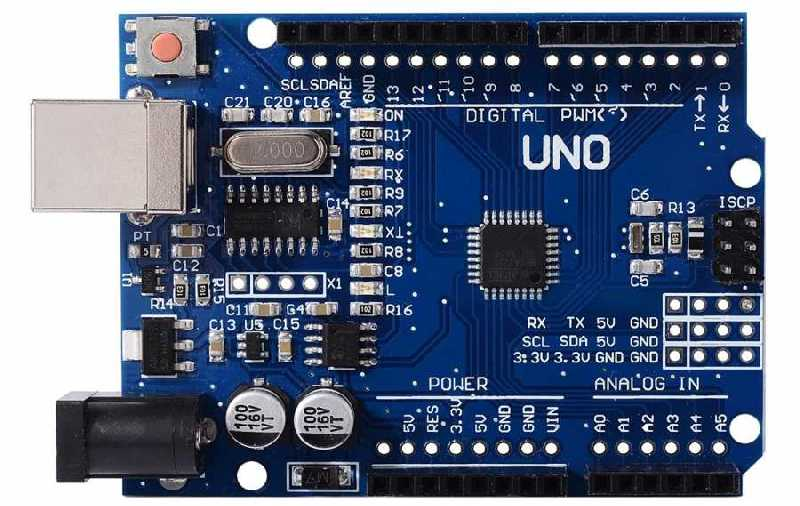
\includegraphics[width=1\textwidth]{../figures/arduino10.jpg}}
  \caption{Ini adalah Arduino}
  \label{arduino}
  \end{figure}

 2. LED 5mm Bening
 \ref{led}
  \begin{figure}[ht]
  \centerline{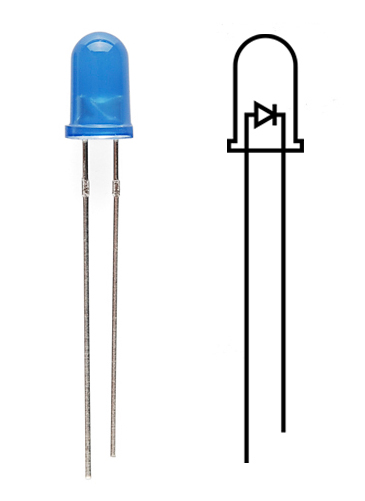
\includegraphics[width=1\textwidth]{../figures/led10.jpg}}
  \caption{Ini adalah Led}
  \label{led}
  \end{figure}

 3. Bread Board
 \ref{brb}
  \begin{figure}[ht]
  \centerline{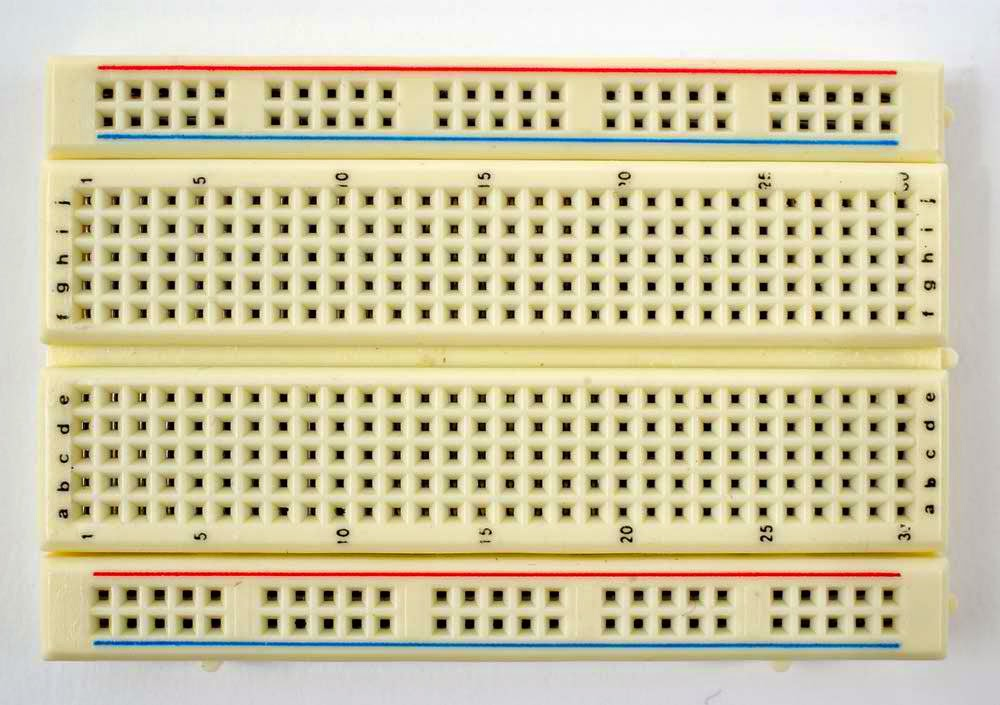
\includegraphics[width=1\textwidth]{../figures/brb.jpg}}
  \caption{Ini adalah BreadBoard}
  \label{brb}
  \end{figure}

 4. Kabel Jumper
 \ref{jumper}
  \begin{figure}[ht]
  \centerline{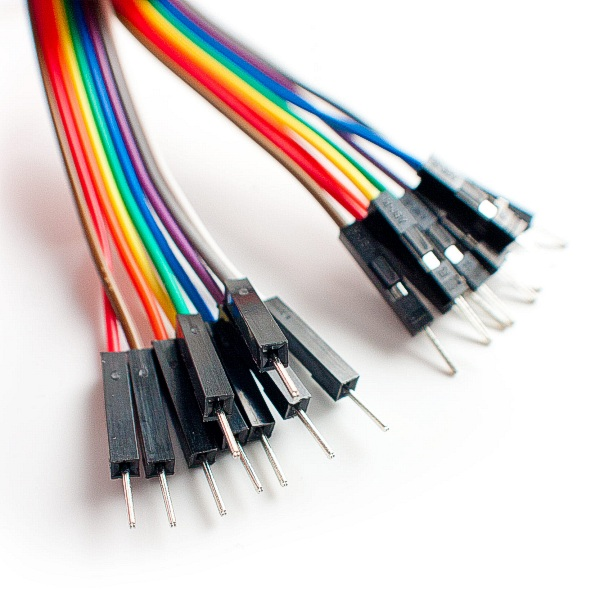
\includegraphics[width=1\textwidth]{../figures/jumper.jpg}}
  \caption{Ini adalah Kabel Jumper}
  \label{jumper}
  \end{figure}

 5. Software IDE Arduino
 \ref{ide}
  \begin{figure}[ht]
  \centerline{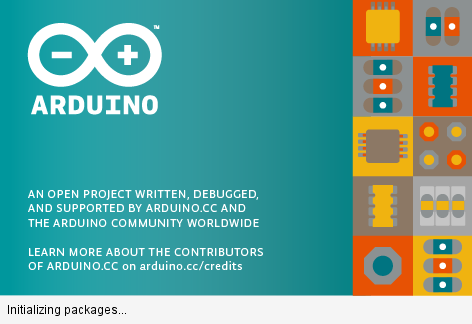
\includegraphics[width=1\textwidth]{../figures/ide.png}}
  \caption{Ini adalah Software IDE}
  \label{ide}
  \end{figure}


\section{Proses Pembuatan}

1 Download dan Instal aplikasi IDE 

2.Rakit semua alat menjadi satu kesatuan 

  \ref{ar2}
  \begin{figure}[ht]
  \centerline{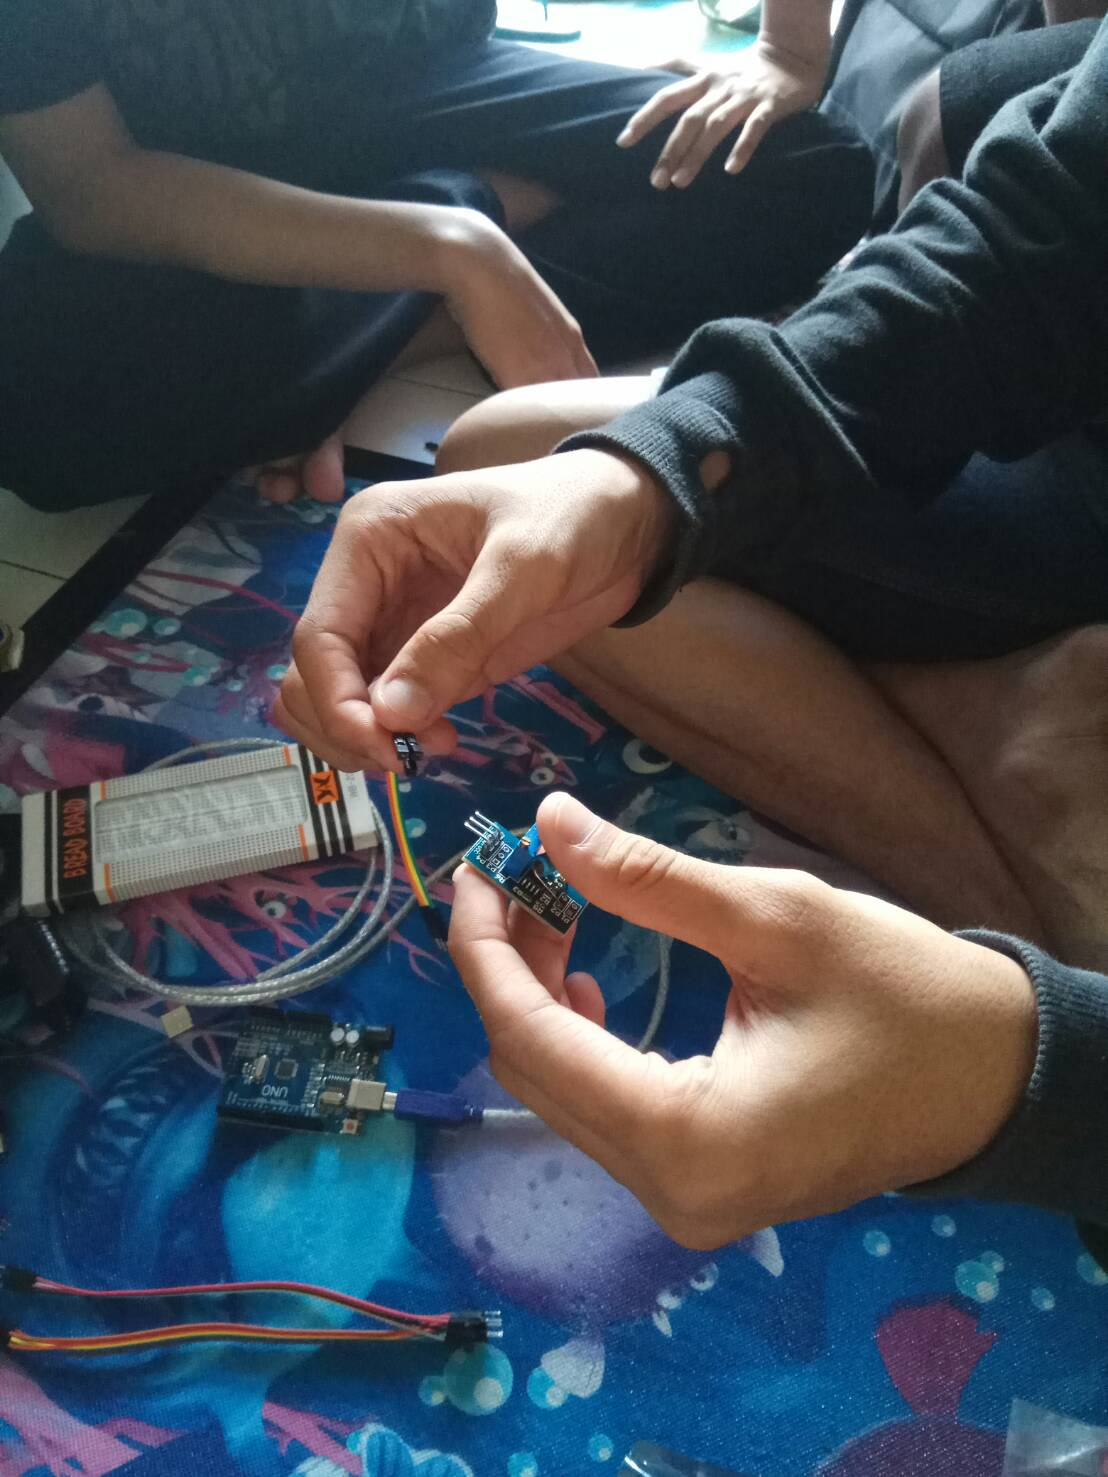
\includegraphics[width=1\textwidth]{../figures/ar2.jpg}}
  \caption{Ini adalah Proses Perakitan}
  \label{ar2}
  \end{figure}

  \ref{ar3}
  \begin{figure}[ht]
  \centerline{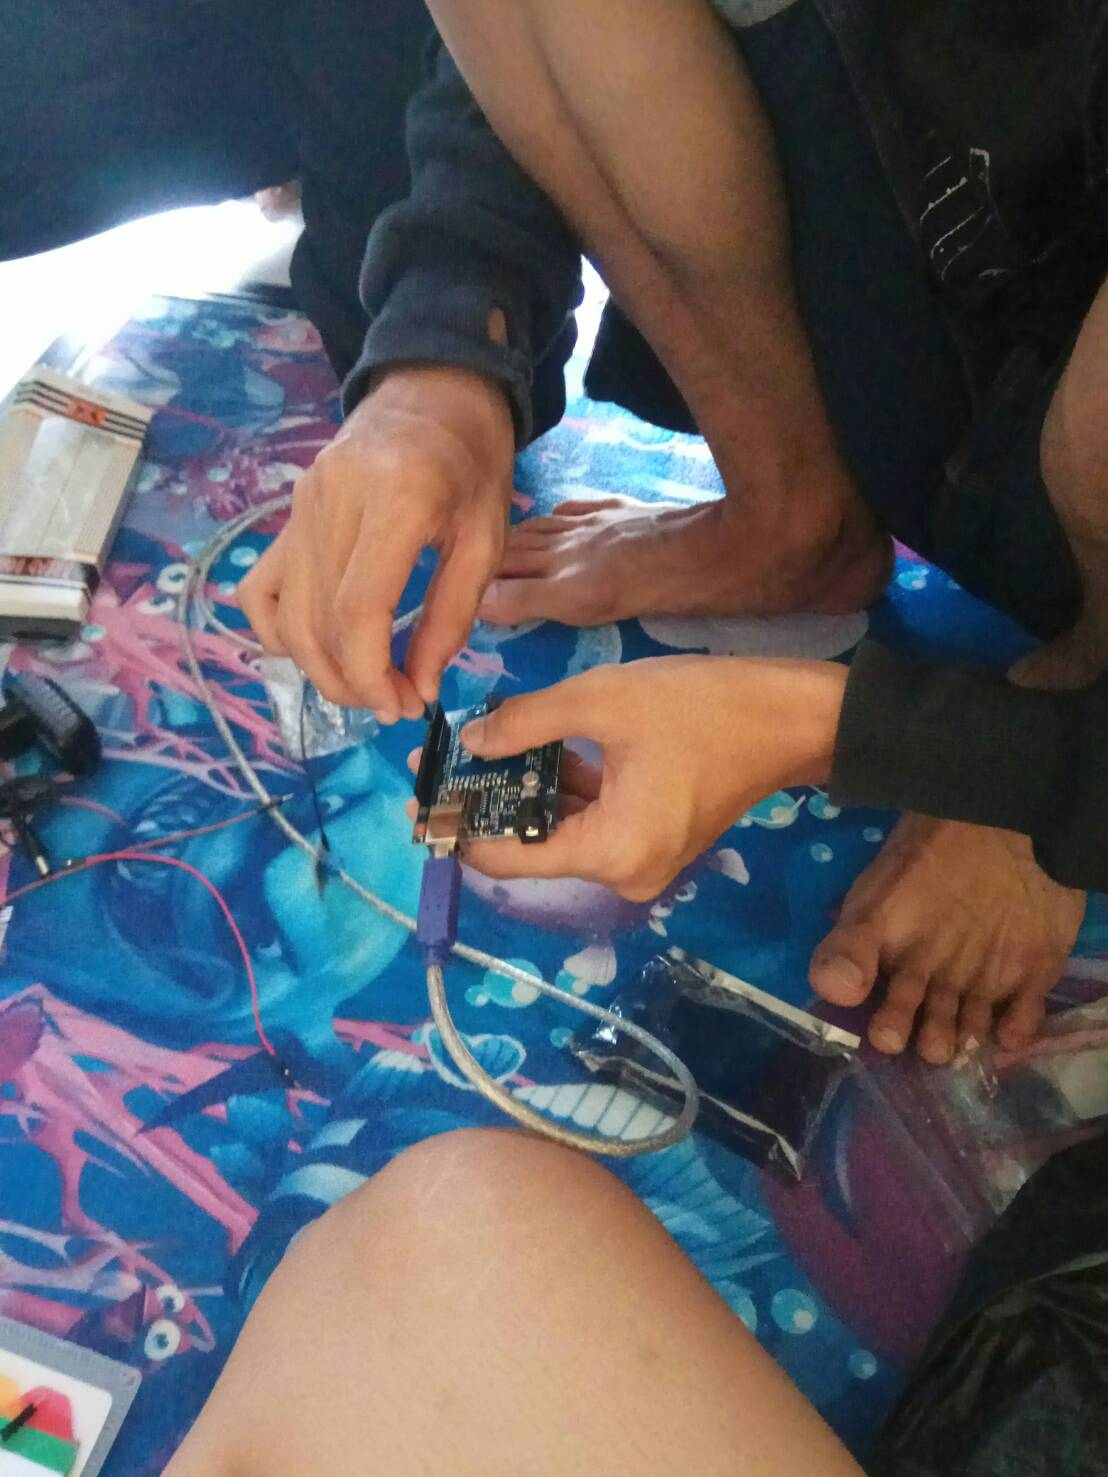
\includegraphics[width=1\textwidth]{../figures/ar3.jpg}}
  \caption{Ini adalah Proses Perakitan}
  \label{ar3}
  \end{figure}

  \ref{ar4}
  \begin{figure}[ht]
  \centerline{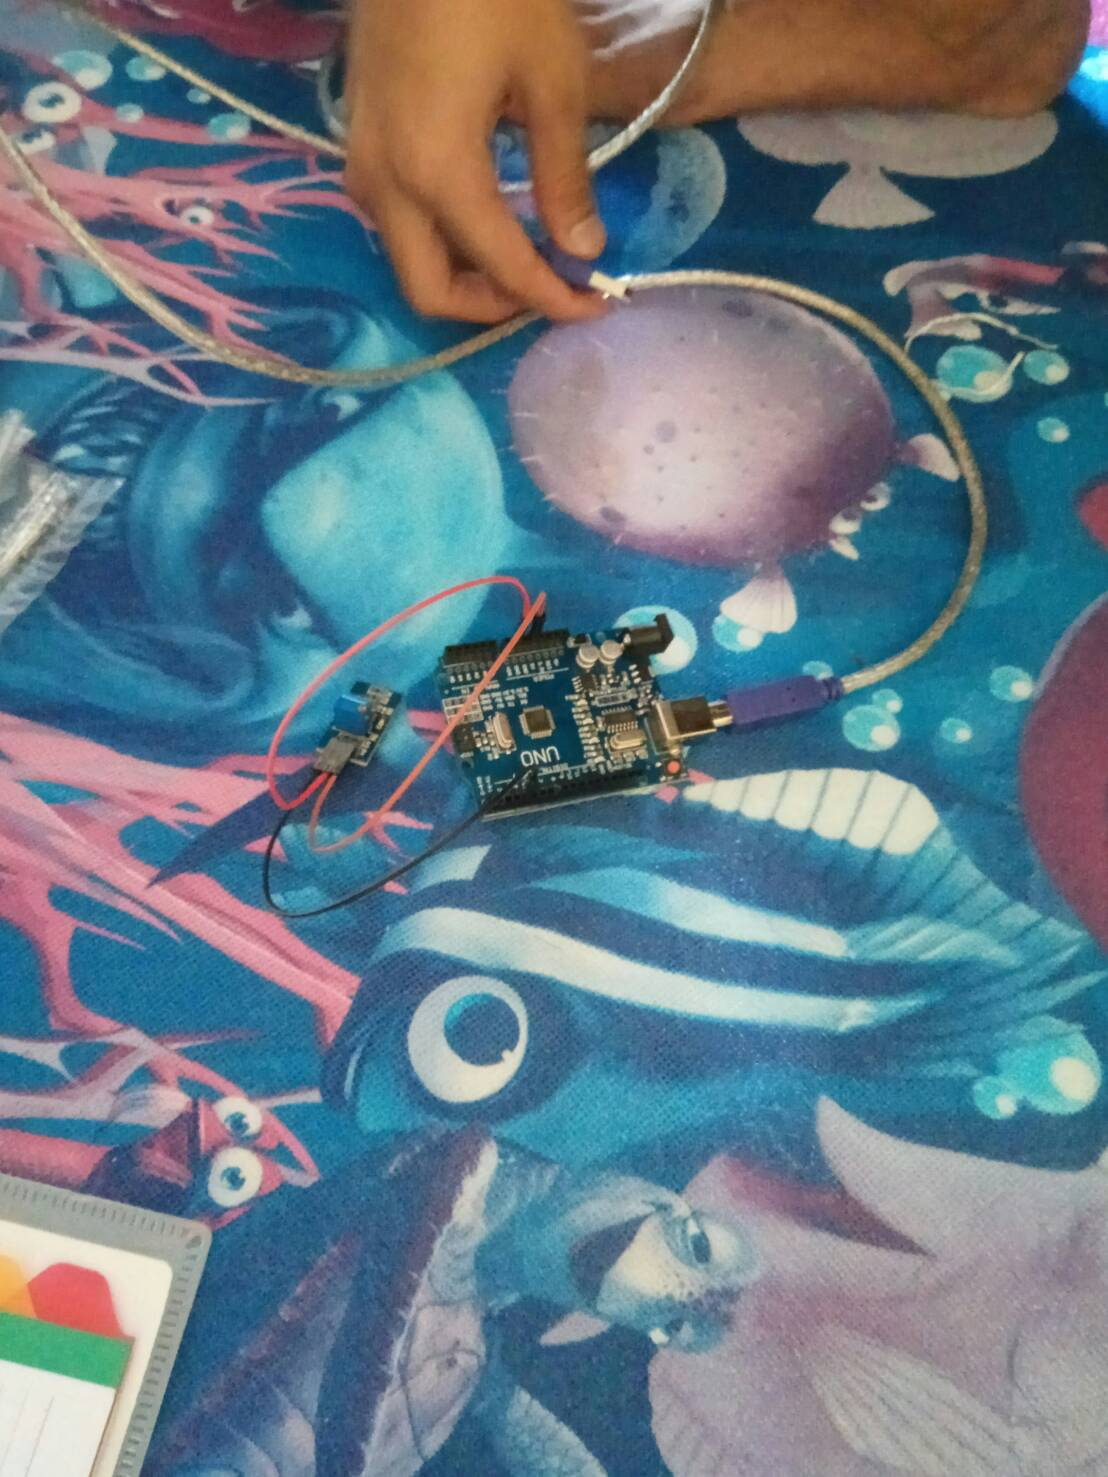
\includegraphics[width=1\textwidth]{../figures/ar4.jpg}}
  \caption{Ini adalah Proses Perakitan}
  \label{ar4}
  \end{figure}

  \ref{ar5}
  \begin{figure}[ht]
  \centerline{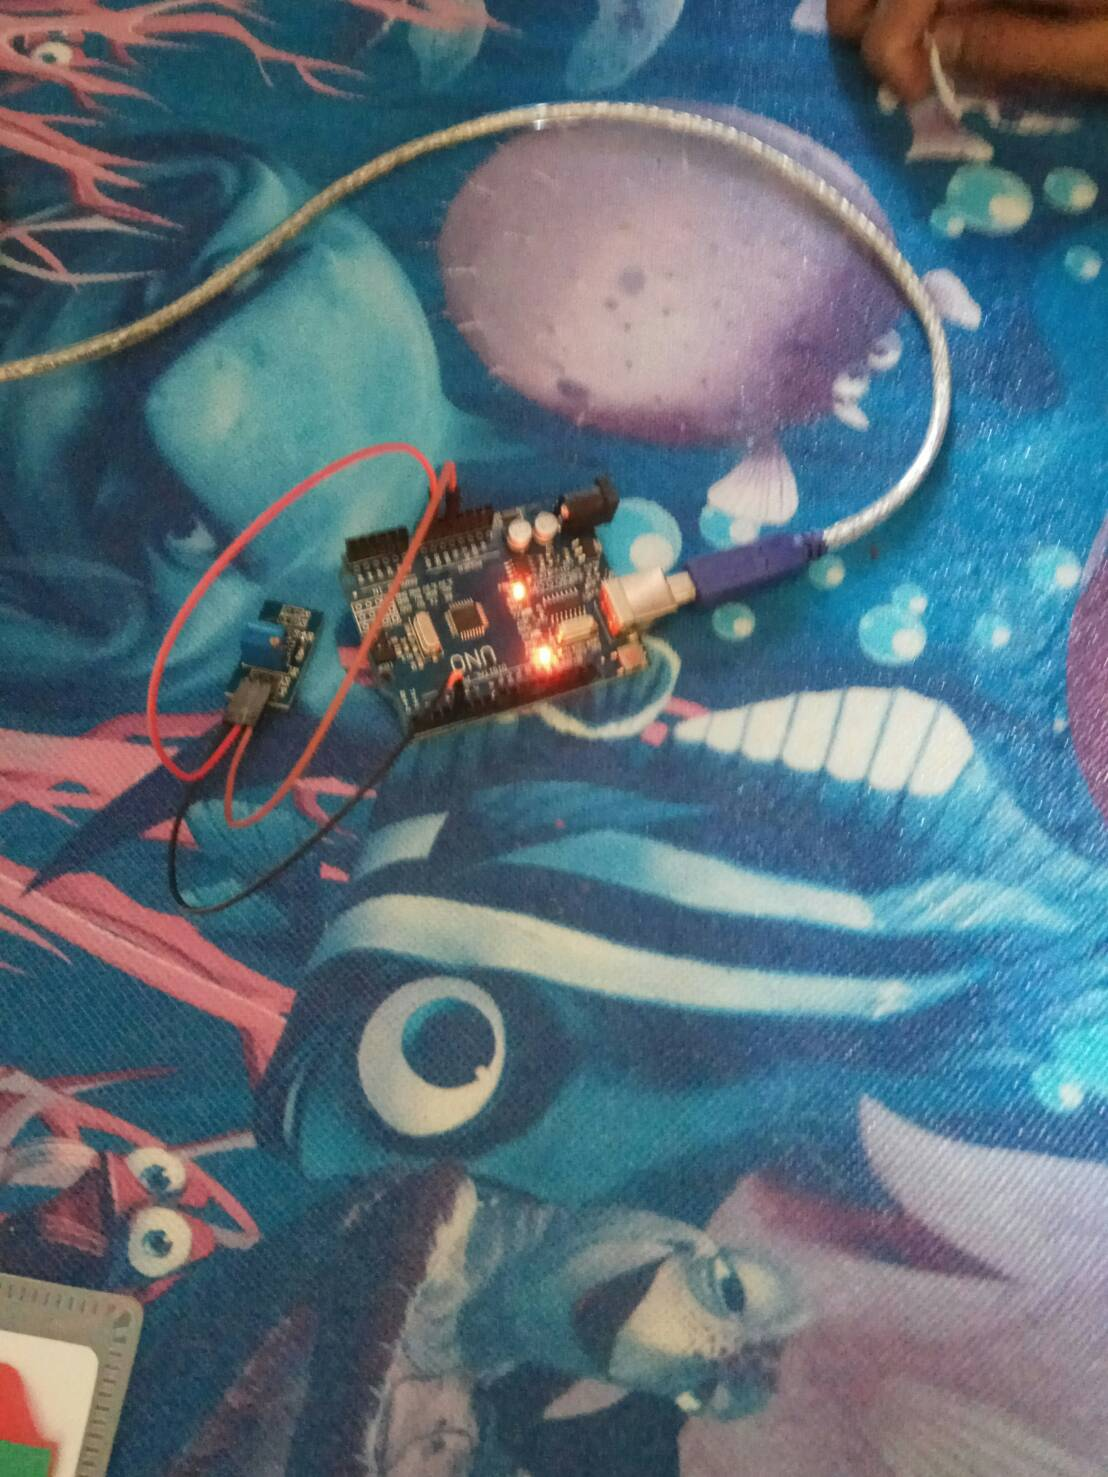
\includegraphics[width=1\textwidth]{../figures/ar5.jpg}}
  \caption{Ini adalah Proses Perakitan}
  \label{ar5}
  \end{figure}

  \ref{ar6}
  \begin{figure}[ht]
  \centerline{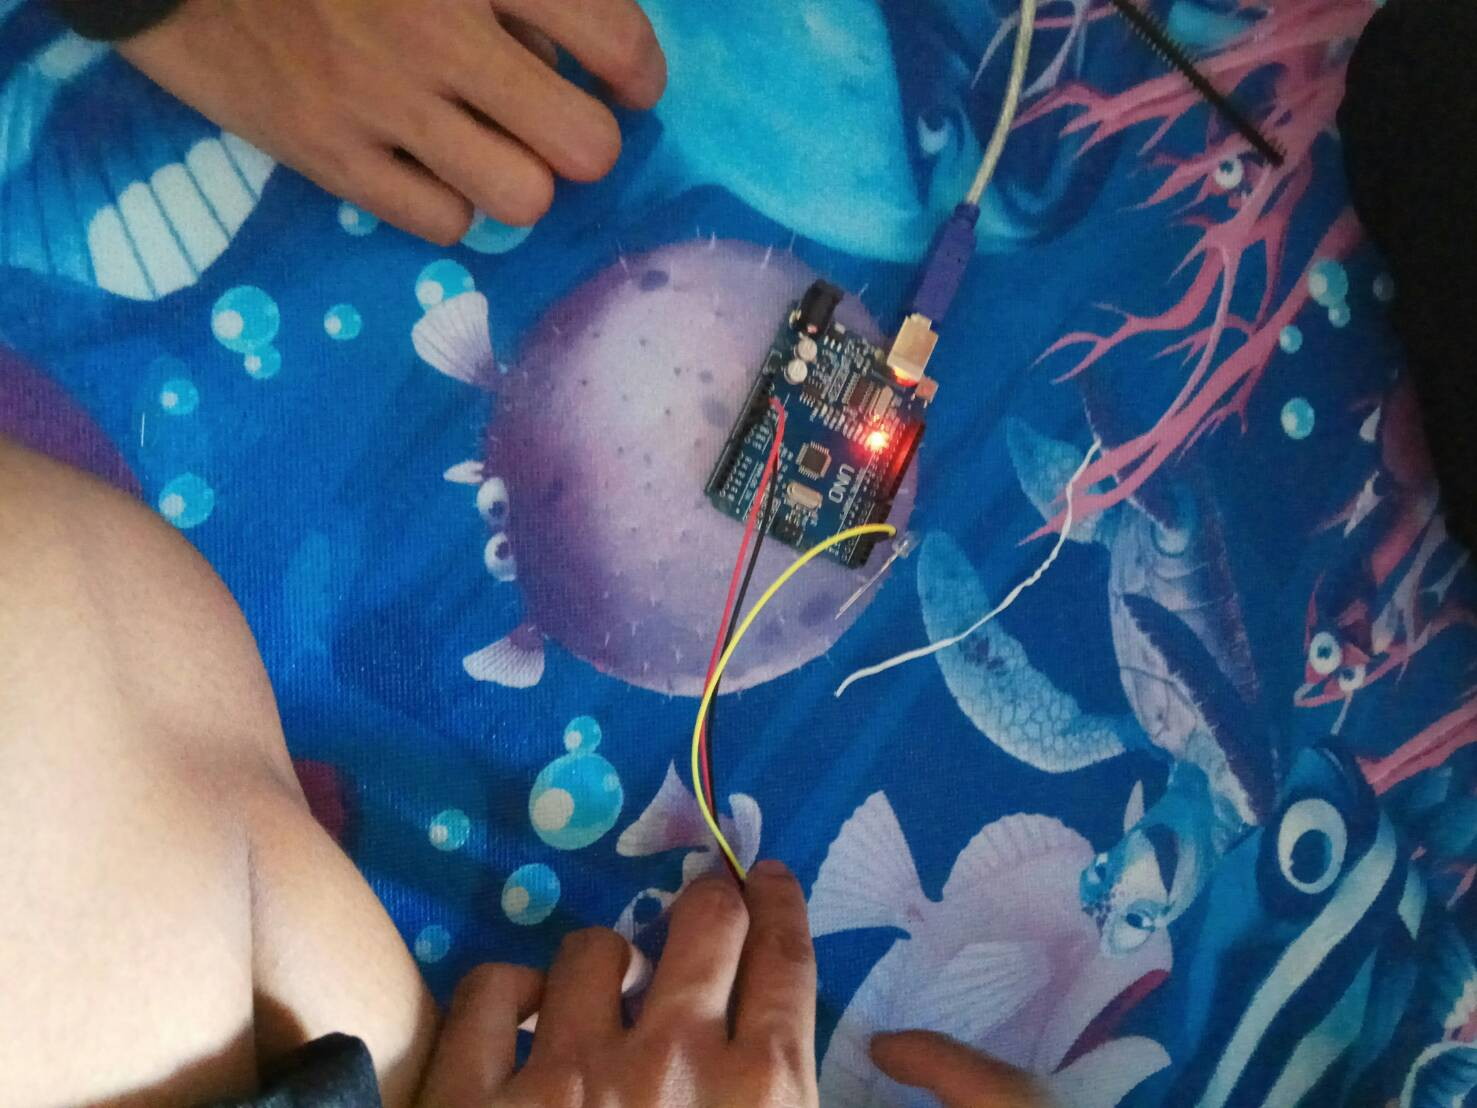
\includegraphics[width=1\textwidth]{../figures/ar6.jpg}}
  \caption{Ini adalah Proses Perakitan}
  \label{ar6}
  \end{figure}

 3. Sambungkan Kabel Printer dengan Laptop

  \ref{ar7}
  \begin{figure}[ht]
  \centerline{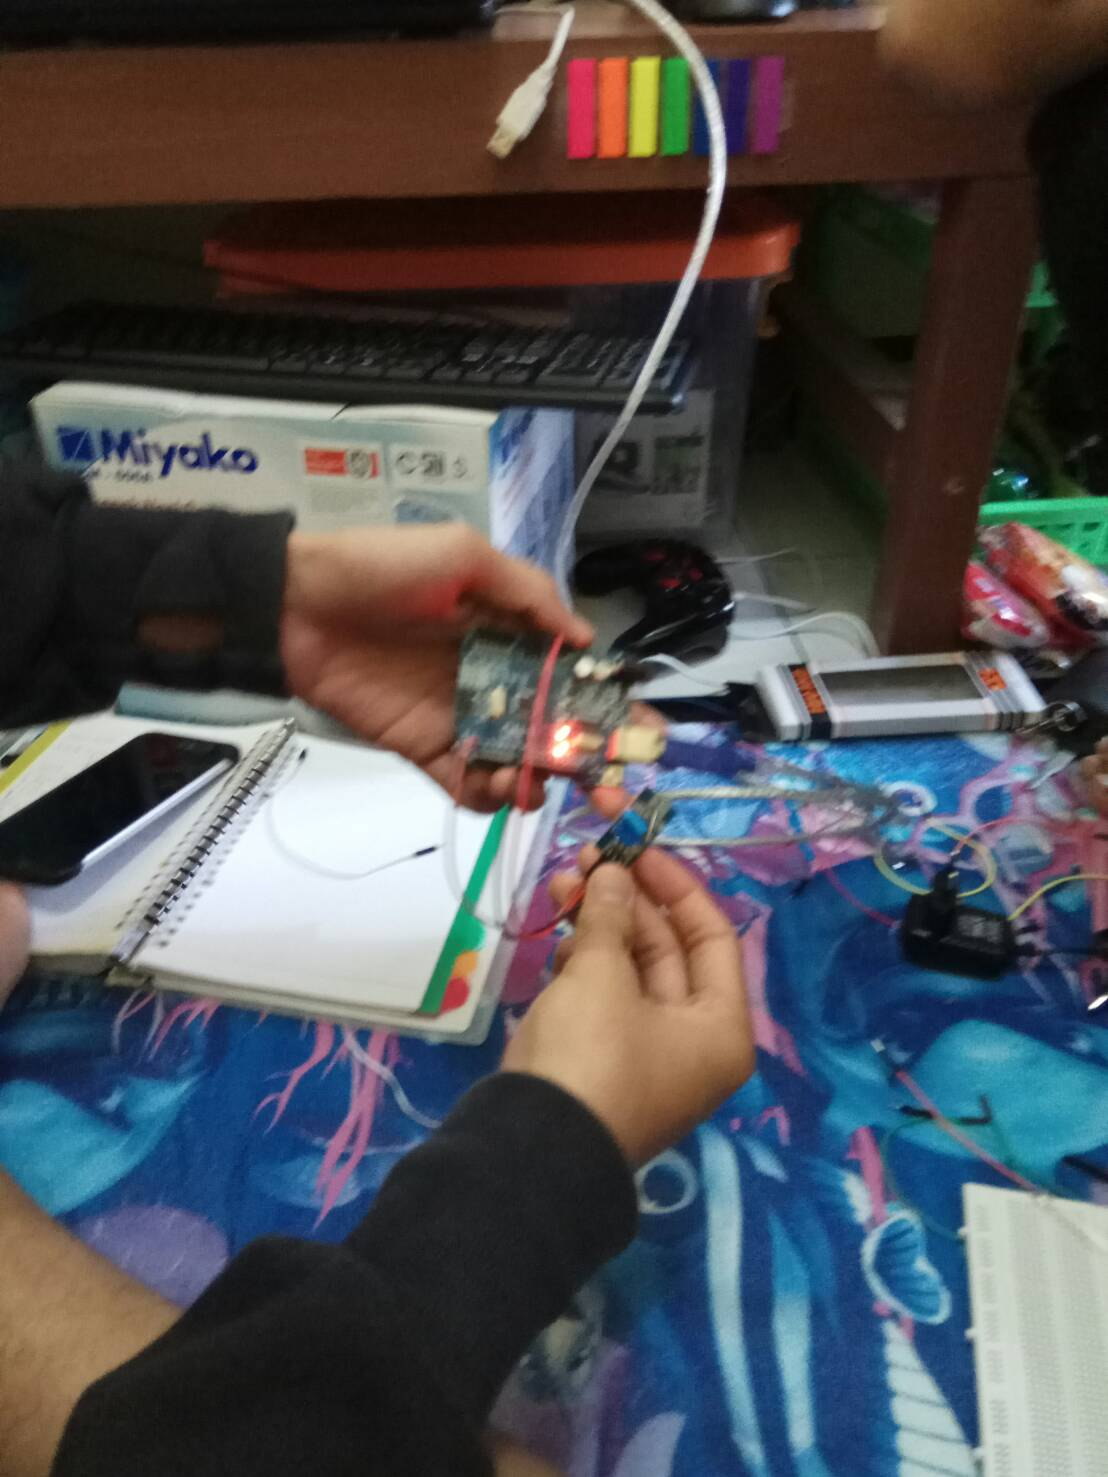
\includegraphics[width=1\textwidth]{../figures/ar7.jpg}}
  \caption{Ini adalah Proses Penyambungan}
  \label{ar7}
  \end{figure}

 4. Lakukan Pengodingan di IDE 
  \ref{ar8}
  \begin{figure}[ht]
  \centerline{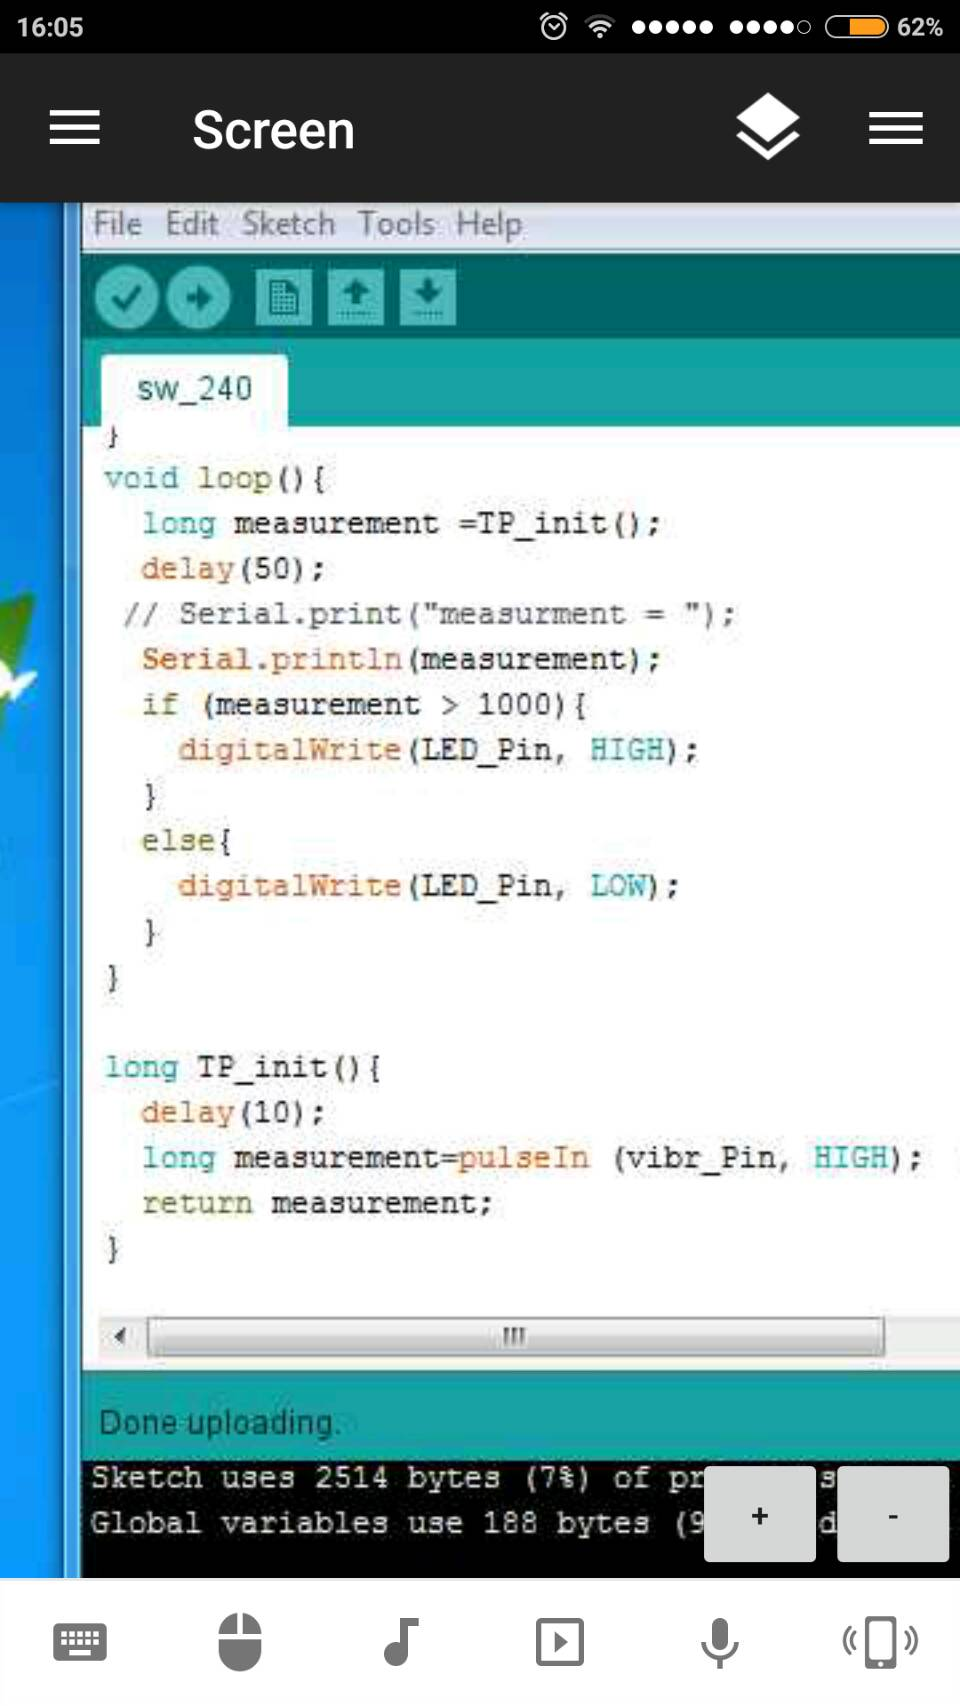
\includegraphics[width=1\textwidth]{../figures/ar8.jpg}}
  \caption{Ini adalah Proses Pengodingan}
  \label{ar8}
  \end{figure}

  \end{document}`````````````````																												